\documentclass[english]{uzhpub}
\usepackage[T1]{fontenc}
\usepackage[utf8]{inputenc}

\begin{document}

%% Titel
\title{Eager Machine Translation}

\subtitle{Master Thesis Description}

\author{Prof. Rico Sennrich, Ph.D.}

\date{\today}

\maketitle

%% Addpart entspricht dem "Kapiteltitel"
%\addpart{Chapter Title}

\section{Introduction}

Neural Machine Translation (NMT) is currently dominated by models that exhibit the following properties:

\begin{itemize}
    \item \textbf{(a) Bipartite structure:} Virtually all methods use so-called \textit{encoder-decoder} models with \textit{attention}. Recurrent, convolutional and self-attentional neural networks have all been proposed as encoder and decoder blocks, but the bipartite structure itself, meaning the division of labour between encoder and decoder, is rarely questioned \cite{jointly.bahdanau2014neural,attentionisallyouneed,pmlr-v70-gehring17a}.
    \item \textbf{(b) Autoregressive inference:} Most NMT models generate translations word by word, conditioning each decision on previously generated words. It is, however, common to \textit{train} non-autoregressively, for instance with Transformer models.
    \item \textbf{(c) Non-simultaneous translation:} During training and inference, the first word of the translation is produced only after seeing the entire input sentence. It is impossible for most models to translate simultaneously. That is, generating the first word of the translation after seeing only a prefix of the input.
\end{itemize}

% There are works that break those conventions in interesting ways.

\noindent This thesis is concerned with \textit{eager translation} \cite{youmaynotneedattention}, a recent model that breaks some of those established conventions. More precisely, it consists of a simple recurrent neural network (RNN) (alternative to \textbf{(a)}) and translates \textit{eagerly}, in the sense that it generates an output word immediately every time it reads a word from the input (alternative to \textbf{(c)}).

% footnote about Gu et a 2017 that break the (b) convention?

\subsection{Is Eager Translation a simultaneous model?}

Translating simultaneously comes at the cost of being unable to revert past decisions. This is because output words are generated at the same time as input words are read. As an example, consider the following scenario:

\begin{quote}
    Input: \hspace{39.5mm} Der Schläger war wütend.\\
    Desired Output: \hspace{24mm} The thug was furious. \\
    Simultaneous Translation Prefix: The racket was \_\_\_
\end{quote}

\noindent After seeing ``Der Schläger war'' as inputs and each time generating the next word of the translation, a simultaneous model would now be presented with ``wütend'' as the next word. This new evidence drastically reduces the likelihood of ``racket'' as the correct translation for ``Schläger''. Yet, a simultaneous model cannot change the word ``racket'' (now a ridiculous translation) to ``thug'' (now a more likely translation). To avoid situations like these, simultaneous models are trusted to \textit{anticipate} future words that they have not yet seen \cite{ma-etal-2019-stacl}.

% comment about what humans do in live translation? repair

% be more precise about epsilon tokens that implicitly allow the model to wait, this reduces load on model: instead of anticipating the correct source word that is in the future, it only has to know when it is unsure

Naturally, anticipating future events may not always be possible. We assume this holds for eager translation models, since \cite{youmaynotneedattention} counteract this apparent shortcoming of their simultaneous model with \textit{beam search}. Beam search is a general searching procedure for sequence generation that considers several hypotheses at the same time. In the example above, beam search could be used to hold on to both ``thug'' and ``racket'' as translations of ``Schläger'', and decide between them later, after seeing more words from the input sentence.

However, beam search arguably removes the simultaneity of translation from the eager model: with beam search, the translation cannot be output until the entire input sentence was read. This effectively \textbf{makes eager translation a non-simultaneous procedure}. 


Additionally, using beam search increases translation latency. The eager model is described as low-latency, but latency increases with beam search (almost linearly with beam size). The beam sizes used for this model are unusually high: tuned on the development set, they are as high as 35 for some experiments. This is unusual, common beam sizes range from 5 to 10. In conventional models, a beam size of 35 does not improve translation quality over beam 5 or 10. If the training data is noisy, a beam of 35 might even lower translation quality \cite{ott2018analyzing}.

% existing text below

%Current Neural Machine Translation (NMT) models employ a so-called encoder-decoder architecture. That is, NMT models commonly include two distinct modules, an encoder and a decoder, such that the encoder translates the input sequence into a list of vectors and the decoder translates this list of vectors into the output sequence, one symbol at a time.

%The encoder and decoder modules typically are modelled as recurrent neural networks (RNNs), a special type of neural network that uses the output of the previous step in the following step to provide the model with information about previous steps of the input sequence. The decoder module uses the output of the encoder and may thus only start once the encoder is finished.

%Additionally, in every step during inference, the decoder returns a set of the top most likely tokens rather than only a single token and subsequently selects the best sequence given this set of tokens from the previous step given again a set of tokens.
%This process is generally known as beam search.

%This leads to an inherently sequential nature in the model architecture that causes training and inference to be computationally very expensive and time consuming. \cite{chung2014empirical,seq2seq.sutskever2014sequence,google.wu2016google,cho2014learning,jointly.bahdanau2014neural,effective.luong2015effective}

%A great body of research to improve the performance and accuracy of neural language models and encoder-decoder architectures has since been conducted in the form of (add some references here, like factorization tricks, conditional computation and what not).
%Research with similar objectives include the application of attention mechanisms in addition to the encoder and decoder modules \cite{jointly.bahdanau2014neural,effective.luong2015effective,attentionisallyouneed}.

%Attention circumvents the issue that traditional neural language models need to represent all relevant information of the source sentence in a single fixed-length vector. An attention mechanism computes a weighted sum of all encoder states in every decoder step and therewith effectively learns to translate and align jointly. These models were shown to be particularly effective on longer sequences \cite{jointly.bahdanau2014neural,effective.luong2015effective}.

%In their most recent work, \cite{attentionisallyouneed} propose a novel architecture that they call the Transformer which is based entirely on attention mechanisms. Their model employs the traditional encoder-decoder architecture but does not use any recurrent networks.

%A big drawback of the transformer architecture is that computing attention is particularly expensive during inference. TODO: elaborate on drawbacks and thus motivation for alternative approaches (You may not need Attention).

%\cite{youmaynotneedattention} propose a model that combines the traditional encoder and decoder steps and eagerly returns a translation after every token of the input sequence. Particularly, \cite{youmaynotneedattention} investigate the potential of neural machine translation models that do not use attention mechanisms.
%Instead, they propose a special pre-processing step that aligns dependencies in the input and target sequences by adding a special $\varepsilon$-token. TODO: elaborate on eager and show example

%That is, in cases in which the translation of a given token of the input sequence follows subsequently in the output sequence, the model learns to return the $\varepsilon$-token and thus delay further translation for another time step. The $\varepsilon$-token can be considered a way for the model to express that it requires more information before making a conclusive decision. That is, the $\varepsilon$-token, effectively, can be considered a \textit{wait}-token.

%\cite{youmaynotneedattention} quantitatively show that their model performs on par with traditional models as introduced by \cite{jointly.bahdanau2014neural}. However, they do not qualitatively or empirically assess the behavior of their model with regards to the $\varepsilon$-tokens. They report that during their experiments translation quality improved if they padded the input sentence with $\varepsilon$-tokens just before the EOS-token but do not elaborate on this further. It may thus be that the $\varepsilon$-token is not helping the model to learn to wait in the case of non-monotonic translations but enables the model to exploit the increased sentence length by simply waiting initially and acquiring multiple tokens of the source sentence before starting to or proceeding to eagerly return translations.

%TODO: show examples of exploit and without exploit

%In the context of waiting and pondering, \cite{act.graves2016adaptive} have introduced an approach that allows recurrent neural networks to learn the number of steps to take between receiving an input and returning an output. TODO: elaborate: XYZ have shown that increased depth leads to more performant networks. On the other hand, deeper networks require more resources during training and inference and more prone to overfit.

%\cite{act.graves2016adaptive} extend the traditional architecture with a state transition model that allows the network to perform a variable number of computation steps for every input it receives. The model learns the number of steps to perform for a given input and therewith learns for which input tokens it requires a deeper computation, it learns for which tokens to wait and ponder, so to speak.

\subsection{Goals}

\textbf{Primary Goal} \\

% \noindent \fbox{\begin{minipage}{\textwidth}
\noindent We identify beam search as a key stumbling block for simultaneous and low-latency eager translation. The primary goal of this work is to lower beam sizes or remove beam search altogether, while not sacrificing translation quality. \\
% \end{minipage}}

\noindent \textbf{Secondary Goals} \\

\noindent As secondary goals, we outline several ways to analyze, improve or extend eager translation. Sorted by priority: \\

\begin{itemize}
    \item \textbf{Analyze anticipation:} we hypothesize that there is an exploit for the model to not actually anticipate future words, by generating \texttt{WAIT} tokens even if anticipation is not necessary.
    \item \textbf{Properties of distillation:} Investigate possible reasons for why distillation boosts greedy translation, such as degree of determinism and monotonicity in the training data.
    \item \textbf{Decoding complexity:} greedy decoding with eager models has low complexity, but unusually high beam sizes increase it again. A detailed analysis could reveal how high beam sizes influence decoding time.
    \item \textbf{Eager Transformer:} recent works have shown that Transformer models can reliably replace RNN language models. This suggests that eager translation is also feasible with a Transformer network. Eager transformers would open up more possibilities, such as fine-tuning from BERT pre-trained weights, or non-autoregressive training for eager models.
    \item \textbf{Learned waiting dynamics:} using \texttt{WAIT} tokens may be too indirect a method to learn proper waiting and anticipation behaviour. To specifically learn when to stop, we could borrow ideas from Adaptive Computation Time (ACT) \cite{act.graves2016adaptive}. A halting unit could be used to decide when to stop reading input tokens. See  \cite{kreutzer2018c} for a similar application of ACT.
\end{itemize}

\section{Proposed Approach}

\subsection{Eager Translation}

% description of eager model?

Eager translation is a simultaneous model proposed by \cite{youmaynotneedattention}. The model does not use attention to get a particular view of an encoded sentence at each decoding step, instead it outputs one word of the translation every time it reads an input word.

The authors introduce a special pre-processing step that aligns words in the source and target sequences. Specifically, special $\varepsilon$ tokens are inserted to avoid source words (in blue) having an alignment to an earlier target word (in red):

\begin{center}
    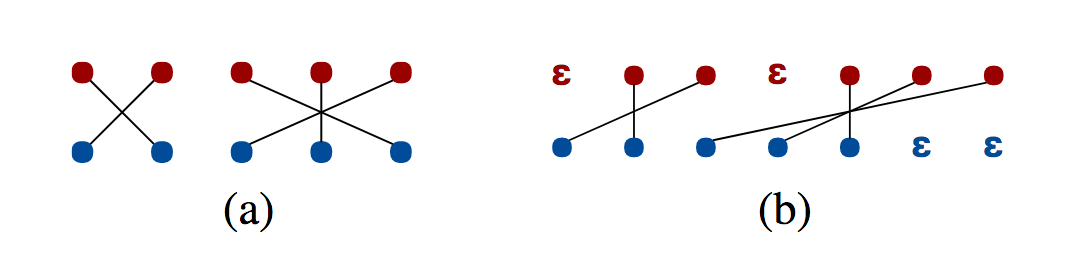
\includegraphics[width=0.5\textwidth]{eager_data.png}
\end{center}

This figure is taken from \cite{youmaynotneedattention}. $\varepsilon$ tokens are also inserted at the end of either sequence to make them equally long. Importantly, $\varepsilon$ is regarded as a regular word in the target vocabulary.

\textit{Eager-feasible pre-processing} is supposed to instil in the model the concept of waiting for more information. That is, in cases in which the translation of a given token of the input sequence follows subsequently in the output sequence, the model learns to return the $\varepsilon$-token and thus delay further translation for another time step. So, effectively, \textbf{the $\varepsilon$-token, can be considered a \texttt{WAIT} token}.

\begin{center}
    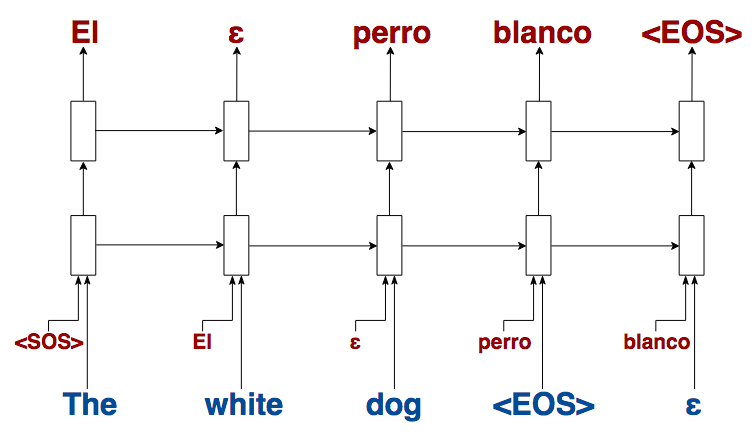
\includegraphics[width=0.5\textwidth]{eager_decode.png}
\end{center}

\subsection{Lower beam size with distillation}

We hypothesize that applying sequence-level knowledge distillation to eager translation may reduce the necessary beam size or remove the need for beam search altogether, while not sacrificing translation quality. 

Knowledge distillation is a procedure where a model (called \textit{student}) is trained to match the predictions of a previous model (called \textit{teacher}) \cite{hinton2015distilling}. \cite{kim2016sequence} have shown that \textit{knowledge distillation} may eliminate the need for beam search in NMT models. Predictions of the teacher model may make the training data less semantically divergent \cite{vyas-etal-2018-identifying} and more deterministic \cite{gu2017non} than the original training data. In a similar context, \cite{gu2017non} have successfully used conventional Transformer models to teach a student model that is non-autoregressive at translation time. A particular advantage of distillation is that the teacher model can be any arbitrary model, including a non-simultaneous model, or an ensemble \cite{freitag2017ensemble}.

\subsection{Analyze anticipation}

% investigate model's anticipation ability / potential exploit

We are particularly interested in the behavior of the model with regards to the $\varepsilon$ tokens and propose to qualitatively assess the effect of the pre-processing method that \cite{youmaynotneedattention} introduce.
Intuitively, it appears that the addition of $\varepsilon$ tokens might enable the model to learn to wait for additional information in cases of non-monotonic translations. Given that their model appears to perform better in configurations where there is a greater number of initial padding tokens and that during their experiments \cite{youmaynotneedattention} have found translation quality to improve if a sentence is padded with $\varepsilon$ tokens before the end-of-sentence-token, it may also be the case that the model simply exploits the $\varepsilon$ tokens to consume additional input tokens initially and thereby counteracts the desired eagerness.

To test whether an eager model uses this exploit, we design an artificial task in which we displace related tokens by a suitable margin and then evaluate the performance of the model and the placement of $\varepsilon$-tokens on these examples.

% The authors report multiple configurations for the padding limit, the source padding injection value and beam size for different numbers of initial padding tokens. The relationship between these values, configurations and the performance of the model remains unclear. Given their unusually large values, we hypothesize that at least the beam size can be reduced with knowledge distillation and propose to investigate the effect of the number of initial padding tokens, the source padding injection value and padding limit in the original model as well as our student model.

\subsection{Properties of distillation}

Distillation demonstrably improves translation performance for greedy decoding. The reasons are not entirely clear, but for simultaneous models in particular, two properties of distilled training data may cause superior translation quality at lower beam sizes:

\begin{itemize}
    \item \textbf{Determinism:} sequences of words generally do not have a deterministic translation. For instance, ``Danke schön'' and ``Vielen Dank'' are both viable translations of ``Thank you'' (example taken from \cite{gu2017non}). Distilled data is believed to be more deterministic because models tend to translate consistently. We design an experiment to quantify the degree of determinism introduced by distillation.
    \item \textbf{Monotonicity:} natural translations are not \textit{eager-feasible}, the ith word in the input might be aligned to any word in the translation. If distillation makes translations more monotone, this could explain improved translation quality. Degree of monotonicity or eager-feasibility could be measured with a word-alignment model.
\end{itemize}

\subsection{Decoding complexity}

Eager translation has a low worst-case asymptotic time complexity of $\mathcal{O}(n+m)$, compared to $\mathcal{O}(n*m)$ for conventional models. However, such an analysis does not consider beam size. Ideal beam sizes for eager models are unusually high, \cite{youmaynotneedattention} report numbers as high as 35. We suggest to analyze in detail the actual complexity for typical sequence lengths instead of asymptotic complexity.

\subsection{Eager Transformer}

Recent works have shown that Transformer models can reliably replace recurrent language models \cite{radford2019language}. Even bi-directional language modeling was shown to be very effective with masked Transformers \cite{devlin-etal-2019-bert}. This suggests that eager translation is also feasible with a Transformer network. Eager transformers would open up more possibilities, such as fine-tuning from BERT pre-trained weights, or non-autoregressive training for eager models.

% talk about implementation effort required?

\subsection{Learned waiting dynamics}

The necessity of beam search for the otherwise simultaneous eager model suggests that \textbf{$\varepsilon$ tokens in the data do not lead to intelligent waiting behaviour}. A different approach to induce the desired waiting dynamics might be to learn it explicitly.

In the context of RNN depth, there is work that describes a mechanism to dynamically adapt the number of RNN layers used for one particular item in the input sequence \cite{act.graves2016adaptive}. \textit{Adaptive computation time} (ACT) adds to the computation graph a \textit{halting unit}, which is a scalar that is incrementally filled up by the model. As soon as the value of the halting unit exceeds a pre-defined threshold, computation for the current time step comes to a halt. To avoid indefinite processing, the model is also encouraged to minimize \textit{pondering time}.

More generally, the concept of a halting unit can be applied in other contexts where a model needs to learn dynamically when to stop in a dynamic way. As an example, \cite{kreutzer2018c} have used ACT to learn optimal word segmentation, meaning that the degree of segmentation is different for every sequence and learned during training.

We propose to repurpose ideas from ACT to learn when to stop reading input words and start outputting words from the translation, by means of a halting unit.

%We furthermore want to investigate the relationship between 
%Additionally, we want to investigate if we can use a student model to produce training data with fewer occurrences of non-monotonic translations and

%The authors report configurations in which they use unusually large beam search values. 

%with large beam size valueswe want to investigate if we're able to reduce 

%We propose to qualitatively assess the effect of adding $\varepsilon$-tokens in the eager translation model that was introduced by \cite{youmaynotneedattention}. 

%The authors report different BLEU performance measures for different numbers of initial padding tokens. Furthermore, \cite{youmaynotneedattention} report multiple configurations for the padding limit, the source padding injection value and beam size for different numbers of initial padding tokens and yet leave no explanation for how and why these configurations were selected.
%Particularly, some configurations appear 

%Particularly, we want to investigate if the model learns to wait in cases of non-monotonic translations or if the model simply exploits the increased sequence length.

%Generally, we want to investigate the relationship between the performance of the model and the number of initial padding tokens, the source padding injection value, the padding limit and the beam size. 

%We propose to apply knowledge distillation on the eager translation model that was introduced by \cite{youmaynotneedattention}. Particularly, \cite{youmaynotneedattention} report 
%We propose to qualitatively assess the effect of adding $\varepsilon$-tokens in the eager translation model that \cite{youmaynotneedattention} introduce. Particularly, we investigate if the model learns to wait in cases of non-monotonic translations or if the model simply exploits the increased sequence length. For this we design and construct an artificial task in which we displace dependent tokens by a suitable margin and then evaluate the performance of the model on these examples.
%Finding and constructing this task will be part of our research.

%We further propose to reproduce the model as outlined by \cite{youmaynotneedattention} and use it as the baseline for our experiments. We then want to extend the model that \cite{youmaynotneedattention} propose with Adaptive Computation Time as introduced by \cite{act.graves2016adaptive} and compare the behavior of the two approaches qualitatively. That is, for more complex parts of sequences, we expect a model with ACT to perform a larger number of computation steps than for simpler tokens and argue that this should reflect in an increased number of iterations for long term dependencies, i.e. non-monotonic translations.

\newpage

\section{Task Description}

\subsection{Lower beam size (primary goal)}

\begin{itemize}
	\item Reproduce model and results from \cite{youmaynotneedattention}
	\item Apply sequence-level knowledge distillation
	\item Measure increasing beam size vs. BLEU for baseline and distillation models
\end{itemize}

\subsection{Do $\varepsilon$-tokens allow a model to learn to wait?}

\begin{itemize}
	\item Design artificial task to assess quality of $\varepsilon$-tokens in \cite{youmaynotneedattention}
	\item Train and evaluate model with artificial task
	\item Qualitatively assess behavior of the model trained on artificial task
\end{itemize}

\subsection{Properties of Distillation}

\begin{itemize}
	\item Quantify degree of determinism and monotonicity in naturally occurring trainig data vs. distilled data
\end{itemize}

\subsection{Decoding complexity}

\begin{itemize}
	\item Compare decoding complexity of a) eager model with a high beam size with b) a conventional encoder-decoder model with low beam size
\end{itemize}

\subsection{Eager Transformer}

\begin{itemize}
	\item implement an eager Transformer, similar to self-attentional language models
	\item use pre-trained BERT weights \cite{devlin-etal-2019-bert} to initialize model and fine-tune weights
\end{itemize}

\subsection{Can ACT be used to learn to wait and ponder in cases of non-monotonic translations?}

\begin{itemize}
	\item Adapt source code from \cite{youmaynotneedattention} and add ACT
	\item Train and evaluate new models
	\item Qualitatively assess behavior of the model trained on artificial task
	\item Compare behavior of the new model with the baseline model
\end{itemize}

\newpage

%\subsection{Evaluation}

% Evaluation in the sense of how do we evaluate translation models?

% Not sure we need this here,
% If you would like to have this section, relevant works:

% Bahdanau 2014, Attention is all you need, you may not need attention, Ma et al 2019, gu et al 2017, kim and rush 2016, hinton et al 2015
% there might be more relevant related works in the related work section of Press & Smith 2018

\section{General Thesis Guideline}

The typical rules of academic work apply and must be followed. At the end of the thesis, a final report has to be written and the work has to be presented. The report should be clearly organized and follow the usual academic report structure.


\section{Tutor}
Mathias M\"uller

\section{Signatures}
\bigskip
\bigskip
\bigskip
\begin{tabular*}{\textwidth}{c @{\extracolsep{\fill}} ccc}
Markus G\"ockeritz  & & Prof. Rico Sennrich, Ph. D.
\end{tabular*}
\newpage

\bibliographystyle{apalike}
\bibliography{proposalbib}
\end{document}
